\documentclass[12pt]{template}
\begin{document}
\section{使用事件描述预测事件参与人数}
\subsection{本章概述}
上一章证明了事件描述对事件参与度有显著的影响,因此,我们便可以通过事件描述来预测参与人数。同时,在第二章预测事件结果的实验中,加入事件描述后成功率有所提高但提高的不是太多,这是因为我们仅采用线性回归来处理文本所导致的。而如果我们能用更精细的方式去处理文本属性,那么分类结果理应有所提高。 所以,接下来本章会提出三种预测器来预测事件描述和事件参与人数之间的关系。这三种预测器分别是线性回归,带卷积层的神经网络和带GRU的神经网络。在实验中,我们将先考察这三类预测器在实际数据集上的表现,然后,这三个预测器将会被用在第二章的预测事件结果的实验,用来代替之前处理文本的方法,以考察预测成功率是否有所提高。

接下来,本章会分别详述这三个预测器。

\subsection{线性回归预测器}
线性回归是最简单的一种回归方法,而且只要二者关系是正相关的,在大多数情况下线性回归也有着不错的效果,因此,这里选择线性回归作为预测算法。同时,线性回归也是本次实验的基线(\textit{baseline})。在实验中,我们并没有采用最传统的线性回归,而是采用了拉索回归。原因是上一章我们假设事件描述对事件参与人数的影响主要由描述中的某些词导致的。所以这里在损失函数中加入$\mathrm{L1}$正则来突出某些词的作用。此预测器及其损失函数如下:
% lasso function
\begin{equation}
argmin\left\{\frac{1}{N}\displaystyle\sum_{i=1}^{N}
(y_i-\beta_0-\displaystyle\sum_{j}\beta_jx_{ij})^2\right\}
\end{equation}
\begin{equation}
subject\ to \quad \displaystyle\sum_{i}|\beta_i|<\alpha
\end{equation}
\begin{equation}
loss\ function: \mathrm{MSE}+\sigma*\sum|\beta|
\end{equation}

在这里,细心的读者可以发现,这里的处理方式和之前的文本处理方式其实是相同的,在实现中,为了与后面两个分类器统一,我们使用了输出维数为1的单层线性神经网络,并采用了L1正则。预测器的输入是序列化后的文本,目标(\textit{target})及输出则是参与人数。


\subsection{带卷积层的神经网络}
在使用线性回归做预测器时,我们假设文本序列中各属性对结果的影响是互相独立,不受出现顺序影响的,即\(d(w|s_0)=d(w|s_0')=d(w)\),其中\textit{w}为词,\(s_0,s_0'\)为不同排列的相同的文本序列,\textit{d}为某个不存在的影响函数。但显然这个假设在现实中是不成立的,在自然语言中,词的出现顺序是非常重要的信息。例如在一段事件描述中,\textit{we will hold the meeting in a church}与\textit{church a in meeting the hold will we}这两句话在上一节的线性规划预测器的眼中是没有区别的,但显然以人的眼光看,第二句话是没有意义的。因此,为了将文本的序列信息纳入考量范围,这里我们参考了seqGan\cite{yu_seqgan:_2016}中判别器的结构,设计了如下了带卷积的神经网络,如图\ref{f21}。判别器的具体处理过程如下。

我们首先将输入文本\(w_0,w_1,...,w_t\)表示成如下形式:
\begin{equation}
S_{1:t}=x_1\oplus x_1\oplus...\oplus x_t
\end{equation}

其中,\(x_i\)为\(w_i\)对应的\textit{k}维词向量\(\subseteq R^k\),\(\oplus\)是拼接符号,\(S_{1:t}\)是一个\(t\times k\)的矩阵。然后我们使用若干个卷积核\(k\subseteq R^{l\times k}\)对窗口大小为\textit{l}中的词进行卷积操作,产生一个新的特征向量。
\begin{equation}
c_i=\rho(w\otimes S_{i:i+l-1}+b)
\end{equation}

\(\otimes\)为按元素乘积(element-wise product)之和,\textit{b}为偏移量,\(\rho\)为非线性函数。在实现中我们可以使用多个相同尺寸的核来进行卷积,然后对得到的不同的\(c_i\)取其中最大的一个,例如图\ref{f21}中第一个卷积核的\textit{l}为3,使用了4个不同的卷积核,即对于相同的窗口一次输出四个结果,然后在这四个结果中取最大值,即为窗口大小为\textit{l}所对应的最终卷积结果。为了得到不同窗口尺寸下的上下文关系,我们也可以使用不同尺寸的核。最后,我们将结果拼接起来,得到处理后的特征向量。送入下一个环节。下一个环节为带隐含层的线性网络,假设得到最终的特征向量为\(\hbar\subseteq R^{k'}\)(图中对应的\textit{k}为9),那么接下来我们对\(\hbar\)进行如下操作。
\begin{equation}
\hbar'=\sigma(w_0\cdot\hbar+b_0)
\end{equation}
\begin{equation}
output = w_1\cdot\hbar'+b_1
\end{equation}

其中\(w_0,w_1\)分别对应第一和第二个蓝色方块,\(\sigma\)为非线性函数,\(\cdot\)为矩阵乘法运算,\(b_0,b_1\)为偏移量。

关于该网络的损失函数,为了最小化预测结果和目标的误差,我们使用了均方误差损失函数($\mathrm{MSE}$),并对最后两个线性神经网络采用了L2正则(公式(\ref{eq1}))。这里采用L2正则的原因是我们希望最后的线性神经网络能尽可能的考虑前面卷积神经网络输出的所有维度,而不是过度的依赖某些维度来做出判断。
\begin{equation}\label{eq1}
loss=\frac{1}{N}\displaystyle\sum_{i=1}^{N}\left\{(y_i-y'_i)^2\right\}+\alpha||w_0^2||+\beta||w_1^2||
\end{equation}
\begin{figure}[htb]
    \centering
    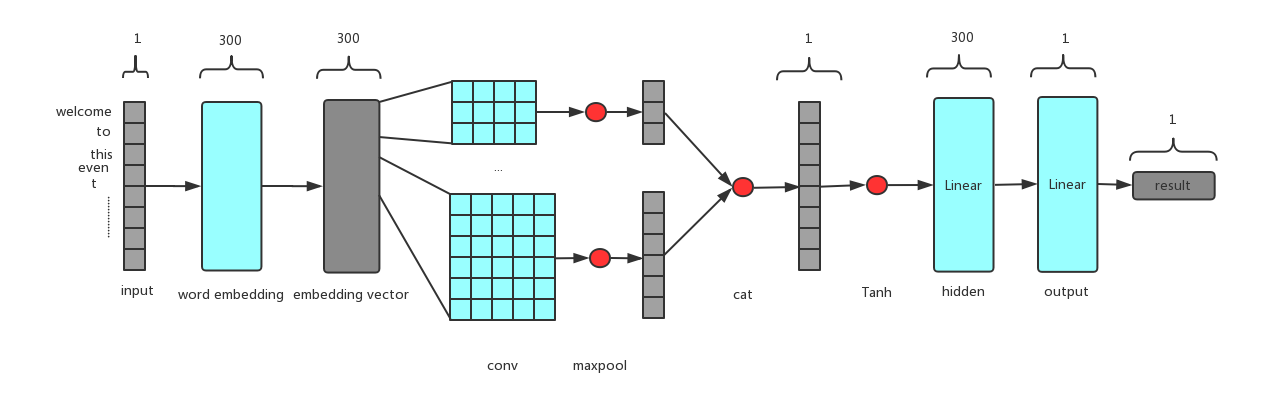
\includegraphics[width=16cm]{conv_ranker.png}
    \caption{带卷积层的神经网络}
    \captionsetup{font=footnotesize,margin=30pt}\caption*{图中灰色的方块表示向量,蓝色的表示网络,红色的圆点表示算符。在计算过程中,输入是文本序列,然后首先经过词向量层转换成词向量,然后进行卷积和池化(max-pooling),将结果拼接起来,然后使用双曲正切(tanh)归一话,最后经过一个带隐含层的线性前馈神经网络输出最终结果。}
    \label{f21}
\end{figure} 

\subsection{带GRU的神经网络}
在上一小节,我们使用了卷积层对原始输入文本转换成的词向量进行了处理,得到了一个新的特征向量。这个过程也可以看成是定义了一个函数\(f:R^{m\times k}\mapsto R^n\),将原本在\(R^{m\times k}\)空间中的样本编码到了\(R^n\)中。这样做的目的是可以方便后续处理,这里我们相当于把一条文本转换成了一个向量,接下来的工作就在这向量上展开了。但如何去找到一个这样的函数\textit{f},则是这种方法成败的关键。在这篇论文中,我们希望\textit{f}有如下的特点:1)能处理序列信息。2)能在转换过程中尽量保留原始信息。3)易于实现。而我们之前使用的卷积层并不完全满足这三个条件。首先,它能处理序列信息,但它处理序列信息的能力来源于窗口大小的设置,因此,合理的设置窗口大小非常重要。而在文本处理中,如何设置窗口大小是件困难的事情。其次,因为池化层的存在,它在转换过程中能保留多少原始信息是存疑的。

而另一种处理时序信息的网络结构循环神经网络,则可以很好的满足上面三个条件。所以近年来这种网络也在自然语言处理上得到了广泛的应用,例如在序列到序列模型中,循环神经网络就常常被用在编码/解码环节。同样在这里,我们使用循环神经网络的特殊形式$\mathrm{GRU}$\cite{DBLP:journals/corr/ChungGCB14}作为编码器。接下来,我们将对GRU进行一个简单的介绍。

\subsubsection{GRU}
GRU(gated recurrent network,图\ref{f22})是为了克服传统的循环神经网络中无法很好的处理远距离依赖而提出的$\mathrm{LSTM}$的一个变体。它相较于$\mathrm{LSTM}$来说更加简单,但仍保持着不错的效果\cite{DBLP:journals/corr/ChungGCB14}。

\begin{figure}[htb]
    \centering
    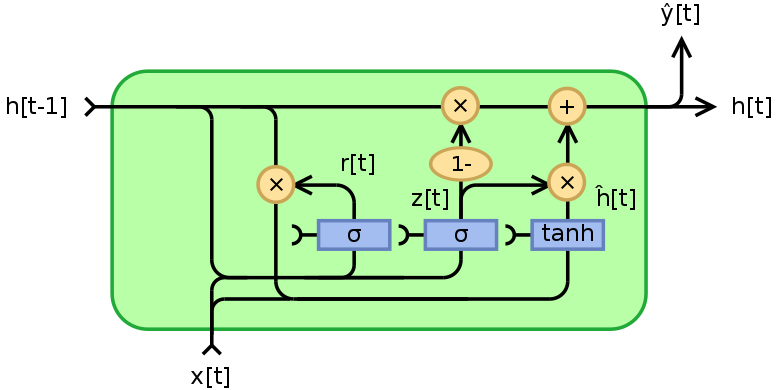
\includegraphics[width=13.5cm]{GRU.png}
    \caption{GRU}
    \captionsetup{font=footnotesize,margin=30pt}\caption*{图中\(z[t]\)为更新门,\(r[t]\)为重置门。\(h[t]\)为当前\textit{t}时刻的隐含状态,橙色的圆点为算符,蓝色方框为某非线性函数}
    \label{f22}
\end{figure}

\subsubsection{GRU的前向传播}
根据图\ref{f22},我们可以得到如下GRU的前向传播公式:
\begin{equation}
z_t=\sigma_z(W_zx_t+U_zh_{t-1}+b_z) 
\end{equation}
\begin{equation}
r_t=\sigma_r(W_rx_t+U_rh_{t-1}+b_r) 
\end{equation}
\begin{equation}
h_t=(1-z_t)\cdot h_{t-1}+z_t\cdot tanh(W_hx_t+U_h(r_t\cdot h_{t-1})+b_h)
\end{equation}

其中,\textit{W,U,b}都是参数。\(x_t\)为输入向量,\(h_t\)为输出向量,\(z_t,r_t\)为更新门和重置门向量。同样的,根据链式法则,我们可以得到其反向传播公式。
\subsubsection{带GRU的神经网络结构}
将之前的神经网络的卷积层替换成本小节介绍的GRU,我们便得到了另一个新的预测器(如图\ref{f23})。可以看出,该预测器的结构与之前的神经网络十分相似,仅在编码环节有所不同。

\begin{figure}[htb]
    \centering
    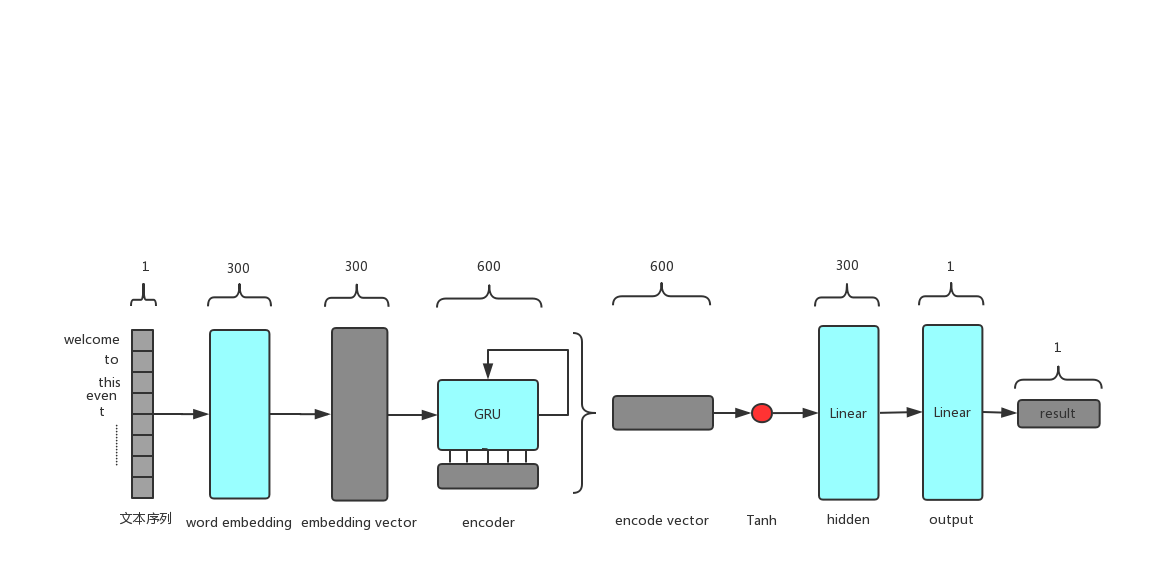
\includegraphics[width=16cm]{gru_ranker.png}
    \caption{带GRU的神经网络}
    \captionsetup{font=footnotesize,margin=30pt}\caption*{图中各色块和圆点的意义同图\ref{f21}。在计算过程中,我们首先将序列转换成词向量,然后使用GRU进行编码,获得一个新的向量(\textit{encode vector}),然后使用双曲正切(\textit{tanh})归一化,最后经过一个带隐含层的线性前馈神经网络输出最终结果。}
    \label{f23}
\end{figure}

\subsection{实验结果}
\subsubsection{预测器的评估}
在本小节中,我们会对本章所介绍的三个预测器在真实的数据集上进行评估。我们所用的数据集来自meetup的LA市,包含超过20万个事件。我们采用百分之八十的事件训练预测器,并用剩下的数据对预测器进行评估。实验结果如图\ref{f24}所示。

\begin{table}[htb]
\caption{\label{t21}网络参数设置}
\centering
\begin{tabular*}{\linewidth}{p{0.333\linewidth}p{0.333\linewidth}p{0.333\linewidth}}
\toprule
    参数         & 带GRU的神经网络 & 带卷积层的神经网络 \\
\midrule
    词向量维度      & 300       & 300       \\
    GRU的\(h_t\)维度   & 600       & 无         \\
    卷积核窗口大小    & 无         & 1,2,3,4,5 \\
    线性神经网络隐层维度 & 300       & 300      \\ 
\bottomrule
\end{tabular*}
\end{table}

\begin{figure}[htb]
	\centering
	\begin{subfigure}{.49\textwidth}
		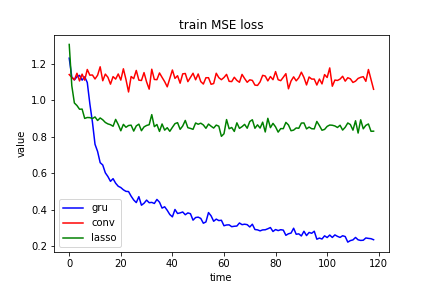
\includegraphics[width=\textwidth]{trainloss.png}
		\caption{train MSE loss}
	\end{subfigure}
%%%%%%%%%%%%%%
	\begin{subfigure}{.49\textwidth}
		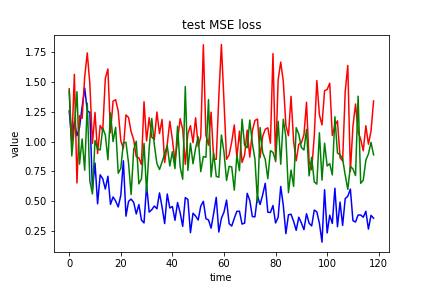
\includegraphics[width=\textwidth]{testloss.png}
		\caption{test MSE loss}
	\end{subfigure}
    \caption{实验结果,其中纵轴为参与人数(对数),横轴为循环次数(×100)}
    \label{f24}
\end{figure} 
从图中我们可以看出,使用GRU作为编码器的神经网络的表现最好,其次是线性预测器,使用卷积层的神经网络表现最糟糕。这点是出乎意料的,原因可能是参数没有调好,以及池化层的存在造成了太多的信息丢失。而另一点值得注意的是尽管GRU在此次实验中的表现最好,但是其结果仍然不是特别理想(从测试环节损失函数的曲线的抖动也可以看出这一点)。这是因为在预测过程中我们仅使用了事件描述这一属性,而没有参考其他属性,例如事件种类,所在组别,举办时间,举办地点,举办者等。属性的缺失限制了这些预测器的上限。如果在预测时加上了这些属性,参考第一章,可以预见准确度应该会有所提升,但由于本文研究对象仅限于事件描述,所以只能到此为止了。 
\subsubsection{使用新的文本处理方式重新训练分类器}\label{train_discrimiator}
本次实验的数据集和分类算法与第二章所采用的方式完全一致,仅在处理文本时使用本章提出的使用GRU作为编码器的神经网络。本次实验仍使用百分之七十的数据作为训练数据,剩余的百分之三十则用来评估分类结果。本次实验使用交叉验证和网格搜索的方式来确定最佳参数,实验结果见表\ref{t2-2}。

\begin{table}[htb] 
    \centering
    \caption{\label{t2-2}使用不同文本处理方法和分类器对预测事件结果的影响}
    \begin{tabular*}{\linewidth}{p{0.2\linewidth}p{0.2\linewidth}p{0.25\linewidth}p{0.25\linewidth}}
\toprule 
分类器&不包含事件描述&使用拉索回归处理文本&使用GRU神经网络处理文本\\
\midrule
Adaboost & 0.762 & 0.791 & 0.801 \\
Decision Tree& 0.763 & 0.786 & 0.811\\
Knn & 0.764 & 0.782 & 0.799 \\
Random Forest & 0.762 & 0.788 & \textbf{0.830} \\
\bottomrule
    \end{tabular*}
\end{table}

实验结果可以看出,使用$\mathrm{GRU}$作为编码器的神经网络来处理事件描述的准确率最高,其次是使用拉索回归处理。排除事件描述作为分类属性的结果最差。所以,在使用了新的文本处理方式后,预测事件成功率的准确度有所提高。这反过来也证明了事件描述在事件成功/事件参与人数上的重要作用。
\subsection{本章小结}
本章提出了三个事件参与人数的预测器,并在真实的数据集上做了实验。实验证明,使用GRU的神经网络在预测事件参与人数的精度上要高于其他两个预测器。这也证明了循环神经网络在处理时序信息上的能力。另外,我们也可以看出实验中就算是最好的结果,其预测精度也不是非常高。这是因为属性缺失导致的。而在这里我们之所以不考虑除事件描述以外的其他属性,是因为本章所设计的预测器在下一章生成事件描述中会作为鉴别器使用,因此无法考虑其他属性。

在下一章,我们将设计一个带变分编码器的端到端的网络作为事件描述生成器,使用本章的带GRU的神经网络作为鉴别器。这两个神经网络将被运用在一个生成对抗网络中,以训练出可以生成新的事件描述的网络模型。
\end{document} 